\documentclass{standalone}
\usepackage{tikz}
\usetikzlibrary{arrows,shapes,matrix,trees,fit,backgrounds,shapes,calc}
% all other packages and stuff you need for the picture
%
\begin{document}
\scalebox{.5}{
  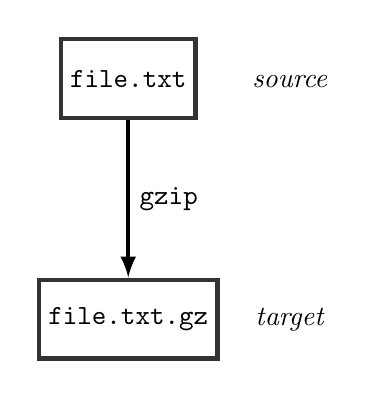
\begin{tikzpicture}[auto, ultra thick,>=latex]
    \tikzstyle{state}=[rectangle,minimum size=1cm, draw=black!80, font=\bfseries, node distance=3cm]
    \tikzstyle{every matrix} = [matrix of nodes, ampersand replacement=\&, align=right, nodes in empty cells, nodes={text height=1.5ex}, minimum width=.4cm]
    \matrix at (0,0)
    {
      \node[state] (txt) {\texttt{file.txt}}; \&[.3cm] \node[right of=txt] {\emph{source}};\\[2cm]
      \node[state] (gz) {\texttt{file.txt.gz}}; \& \node[right of=gz] {\emph{target}};\\
    };
    \draw (txt) edge[->] node[right] (txt) {\texttt{gzip}} (gz);
  \end{tikzpicture}
}
\end{document}

%%% Local Variables: 
%%% mode: latex
%%% TeX-master: t
%%% End: 
